\documentclass[aspectratio=169]{beamer}

% --- minimalist theme matching the original deck (tan/gold accent on white) ---
\usetheme{default}
\usefonttheme{professionalfonts}
\setbeamertemplate{navigation symbols}{}
\usepackage[T1]{fontenc}
\usepackage{amsmath,amssymb}
\usepackage{graphicx}
\graphicspath{{../img/}}

\definecolor{tan}{RGB}{193,154,107}
\definecolor{ink}{RGB}{40,40,40}
\setbeamercolor{structure}{fg=tan}
\setbeamercolor{frametitle}{fg=ink}
\setbeamercolor{title}{fg=ink}
\setbeamercolor{itemize item}{fg=tan}
\setbeamercolor{itemize subitem}{fg=tan}
\setbeamerfont{frametitle}{size=\LARGE}
\setbeamertemplate{frametitle}{\vspace{4mm}\insertframetitle\par}

% section divider with the tan right panel, like the original outline slides
\newcommand{\sectiondivider}[3]{%
\begin{frame}[plain]
  \begin{columns}
    \begin{column}{0.52\textwidth}
      \small #2
      \vfill
      {\scriptsize\color{gray} #3}
    \end{column}
    \hfill
    \begin{column}{0.48\textwidth}
      \colorbox{tan}{\begin{minipage}[t][0.86\paperheight][c]{\textwidth}
        \hspace{4mm}{\color{white}\Huge\textbf{#1}}\\[2mm]
      \end{minipage}}
    \end{column}
  \end{columns}
\end{frame}}

\title{\textbf{Neuro-symbolic approaches to the SAT problem}}
\subtitle{Pattern Recognition \& Reinforcement Learning\\(survey with coding project)}
\author{Donato Meoli}
\date{}

\begin{document}

{\setbeamertemplate{footline}{}
\begin{frame}[plain]
  \vspace{1.2cm}
  \hfill\begin{minipage}{0.7\textwidth}\raggedleft
  {\color{tan}\rule{2pt}{2.2cm}}\hspace{3mm}
  \begin{minipage}{0.82\textwidth}\raggedright
    {\Huge Neuro-symbolic\\ approaches to\\ the SAT problem}\\[3mm]
    {\large Pattern Recognition \&\\ Reinforcement Learning\\ (survey with coding project)}\\[8mm]
    {\normalsize Donato Meoli}
  \end{minipage}
  \end{minipage}\hfill\,
\end{frame}}

% ------------------------------------------------------------------ SAT problem
\begin{frame}{SAT Problem}
  \begin{itemize}
    \item \textbf{SAT}: is there an assignment satisfying a Boolean formula (CNF)?
          First problem proven NP-complete; core of verification, planning, synthesis.
    \item Modern solvers are \textbf{CDCL}: decide a variable, unit-propagate, on a
          conflict learn a clause and backtrack.
    \item The \textbf{branching heuristic} (e.g.\ VSIDS) picks the decision variable
          --- a natural target for machine learning.
    \item \emph{This project}: survey + implementation of two neuro-symbolic
          branching approaches, modernised to a single PyTorch stack and
          reproduced.
  \end{itemize}
\end{frame}

% ================================================================== NeuroSAT
\sectiondivider{NeuroSAT}{%
  \begin{itemize}
    \item NeuroSAT
    \item Background
      \begin{itemize}\item Message Passing Neural Networks (MPNNs)\end{itemize}
    \item Model \item Training \item Results
  \end{itemize}}{(ISPR -- survey)\\[2mm]
  Selsam et al., \emph{Learning a SAT Solver from Single-Bit Supervision}.\\
  Gilmer et al., \emph{Neural Message Passing for Quantum Chemistry}.}

\begin{frame}{NeuroSAT}
  \begin{itemize}
    \item \textbf{Goal}: can a neural network learn to solve SAT?
    \item An MPNN trained \emph{only} as a SAT/UNSAT classifier (one-bit
          supervision) nonetheless learns to find satisfying assignments.
    \item At test time, for a satisfiable instance the network guesses UNSAT with
          low confidence until it ``finds'' a solution, then converges to SAT.
    \item Survey item only --- not implemented here, but the graph view it
          introduces is the basis of Graph-Q-SAT.
  \end{itemize}
\end{frame}

% ================================================================== AlphaZeroSAT
\sectiondivider{AlphaZeroSAT}{%
  \begin{itemize}
    \item AlphaZeroSAT
    \item Background
      \begin{itemize}\item Monte Carlo Tree Search (MCTS)\end{itemize}
    \item Model \item Training \item Results
  \end{itemize}}{(ISPR + RL -- survey with coding)\\[2mm]
  Wang \& Rompf, \emph{From Gameplay to Symbolic Reasoning: Learning SAT Solver
  Heuristics in the Style of Alpha(Go) Zero}.}

\begin{frame}{AlphaZeroSAT --- Model}
  \begin{itemize}
    \item \textbf{Goal}: can Alpha(Go)Zero learn a branching heuristic for SAT?
    \item State: CNF as a fixed-size \textbf{clauses\,$\times$\,variables} matrix,
          entries encoding literal polarity ($(1,0)$ / $(0,1)$).
    \item A \textbf{CNN} with a policy head $\pi$ (over $2\,n_{\text{var}}$ actions)
          and a value head $v\in[-1,1]$; invalid actions are masked.
    \item MiniSat is extended into a \emph{game} env supporting MCTS
          \textbf{simulations} (hypothetical roll-outs without mutating the state).
  \end{itemize}
\end{frame}

\begin{frame}{AlphaZeroSAT --- Training}
  \begin{itemize}
    \item \textbf{Self-play}: MCTS, guided by $(\pi,v)$, produces improved visit
          distributions; tuples (state, MCTS-policy, outcome) are stored.
    \item \textbf{Supervised} update with the AlphaZero loss
          \[\mathcal{L}= -\textstyle\sum_a \pi^{\text{MCTS}}_a\log\pi_a + (z-v)^2 + c\lVert\theta\rVert_2^2 .\]
    \item Dataset: uniform-random 3-SAT, $20$ vars / $91$ clauses
          (\texttt{uf20-91}), 32 train / 200 test.
  \end{itemize}
\end{frame}

\begin{frame}{AlphaZeroSAT --- This work (modernisation)}
  \begin{itemize}
    \item Ported TensorFlow~1.x $\rightarrow$ \textbf{PyTorch}: networks
          (\texttt{models\_torch}), trainer (\texttt{alphazero\_torch}), self-play
          driver (\texttt{main\_torch}).
    \item \textbf{Removed the GSL dependency} from the C++ env: Dirichlet noise
          reimplemented with C++11 \texttt{<random>} $\Rightarrow$ builds with only
          \texttt{g++}/\texttt{zlib}, no \texttt{sudo}.
    \item Cleaned the fork (dropped unused OpenAI-baselines code), \textbf{runs
          end-to-end} locally on the modern stack.
    \item \emph{Limitation}: the fixed-size CNN does not generalise across problem
          sizes --- motivating the graph approach.
  \end{itemize}
\end{frame}

% ================================================================== GraphQSAT
\sectiondivider{GraphQSAT}{%
  \begin{itemize}
    \item GraphQSAT
    \item Background
      \begin{itemize}\item Deep Q-Learning (DQN)\item Graph Neural Networks (GNNs)\end{itemize}
    \item Model
    \item Graph Attention Networks (GATs)
    \item Training \item Results
  \end{itemize}}{(ISPR + RL -- survey with extra coding)\\[2mm]
  Kurin et al., \emph{Can Q-Learning with Graph Networks Learn a Generalizable
  Branching Heuristic for a SAT Solver?}\\ Battaglia et al., \emph{Relational
  inductive biases, deep learning, and graph networks}.}

\begin{frame}{Graph-Q-SAT --- Model}
  \begin{itemize}
    \item \textbf{Goal}: can DQN with a GNN learn a \emph{generalizable} branching
          heuristic?
    \item State: \textbf{bipartite graph} (variable / clause nodes); node features
          2-D one-hot, edge features = literal polarity, empty global.
    \item $Q$-function: \textbf{encode--process--decode} graph network; action =
          $\arg\max$ $Q$ over variable nodes.
    \item Reward $-p$ per step, $0$ at termination; metric = \textbf{MRIR}
          (median MiniSat-iters / model-iters).
  \end{itemize}
\end{frame}

\begin{frame}{GAT-Q-SAT --- attention variant (extra coding)}
  \begin{itemize}
    \item Inject \textbf{Graph Attention} (\texttt{GATConv}, edge-aware, multi-head)
          into the core message-passing block.
    \item Attention weights neighbouring clauses/variables --- useful when the
          instance has an exploitable sub-structure.
    \item Same DQN training; toggled with \texttt{--use\_attention}.
    \item \emph{Note}: the field later moved to attention/Graph-Transformers
          (NeuroBack, ICLR'24) --- this variant anticipated that direction.
  \end{itemize}
\end{frame}

\begin{frame}{Results --- graph colouring (MRIR vs model decisions)}
  \begin{columns}
    \begin{column}{0.5\textwidth}\centering
      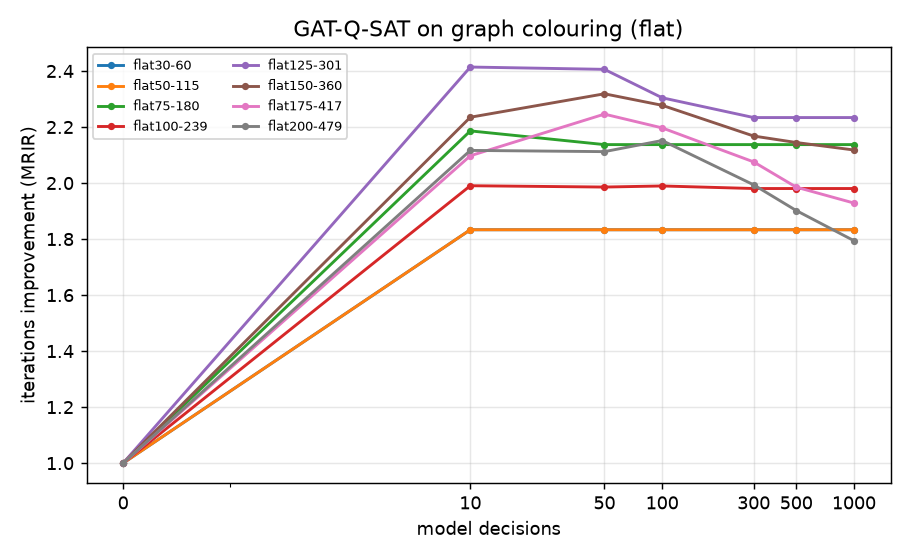
\includegraphics[width=\textwidth]{gatqsat.png}\\[-1mm]
      {\scriptsize GAT-Q-SAT: strong \& stable, also on large instances}
    \end{column}
    \begin{column}{0.5\textwidth}\centering
      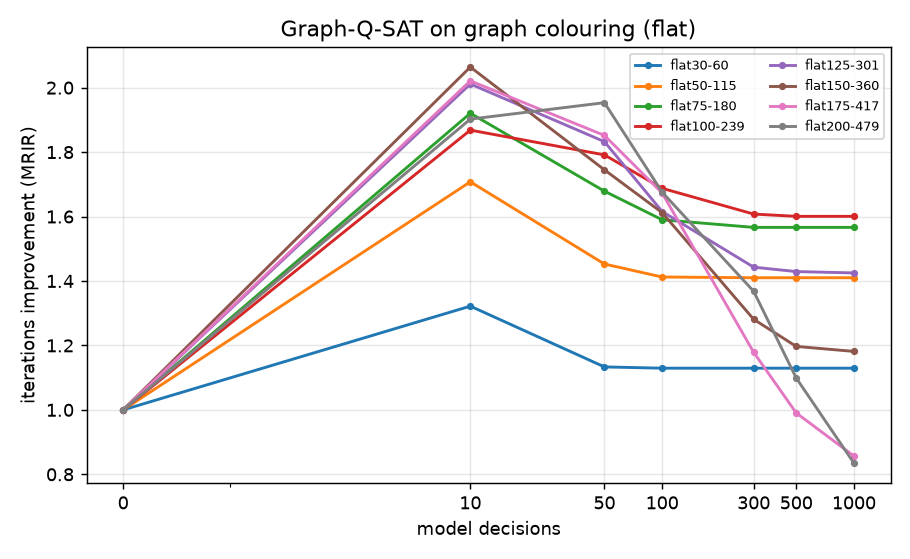
\includegraphics[width=\textwidth]{graphqsat.png}\\[-1mm]
      {\scriptsize Graph-Q-SAT: degrades on large instances at high caps}
    \end{column}
  \end{columns}
  \vspace{1mm}
  {\footnotesize Generated locally from \texttt{runs/*/*.tsv} (\texttt{make\_plots.py}) --- no more Google Sheets.}
\end{frame}

\begin{frame}{Results --- random 3-SAT and solving time}
  \begin{columns}
    \begin{column}{0.5\textwidth}\centering
      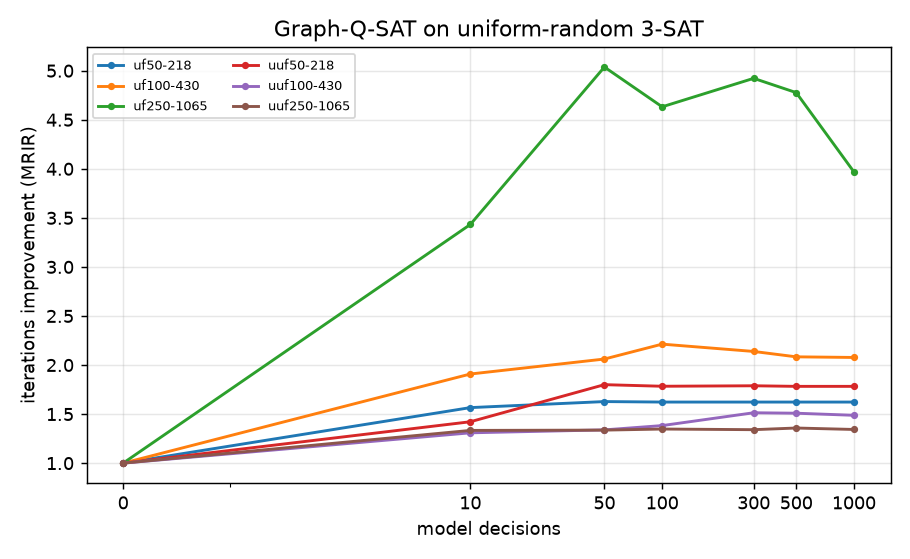
\includegraphics[width=\textwidth]{graphqsat_random.png}\\[-1mm]
      {\scriptsize On random 3-SAT, plain Graph-Q-SAT is strongest ($\sim$5$\times$)}
    \end{column}
    \begin{column}{0.5\textwidth}\centering
      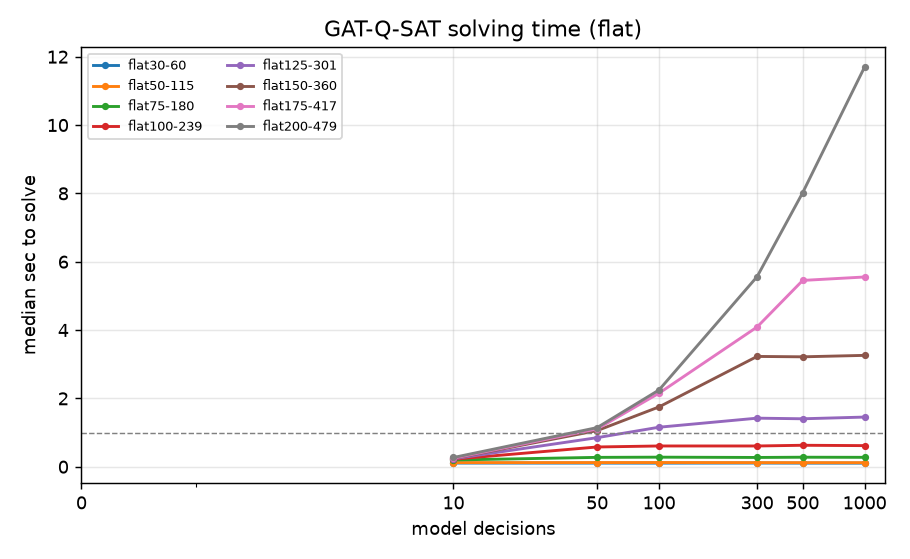
\includegraphics[width=\textwidth]{gatqsat_time.png}\\[-1mm]
      {\scriptsize Wall-clock time vs.\ model decisions}
    \end{column}
  \end{columns}
  \vspace{1mm}
  \textbf{Finding}: attention helps where there is structure to infer (graph
  colouring); on near-uniform random SAT it does not.
\end{frame}

\begin{frame}{Results --- exact reproduction (this work)}
  \begin{itemize}
    \item Re-ran the \emph{original trained checkpoints} on the modern stack
          (latest torch / PyTorch~Geometric / numpy~$\geq$2 / gymnasium).
    \item MRIR matches the committed logs \textbf{exactly} --- e.g.\
          \texttt{flat30-60}, cap 500:
  \end{itemize}
  \begin{center}\small
  \begin{tabular}{lcc}
    \hline
    Model & MRIR (median) & committed \\ \hline
    Graph-Q-SAT & 1.833 & 1.833 \\
    GAT-Q-SAT   & 1.667 & 1.667 \\ \hline
  \end{tabular}
  \end{center}
  \begin{itemize}
    \item Drop-in changes only (scatter, env construction, GATConv key remap) ---
          \textbf{semantics preserved}.
  \end{itemize}
\end{frame}

% ================================================================== Conclusions
\begin{frame}{Conclusions}
  \begin{itemize}
    \item Two neuro-symbolic SAT methods modernised to one self-contained
          \textbf{PyTorch} stack; brittle deps (TF1.x, GSL,
          torch-scatter/sparse, pinned gym) removed.
    \item Results \textbf{reproduced exactly}; figures regenerated locally.
    \item \textbf{Graph attention} helps on structured problems (graph colouring),
          not on uniform-random SAT.
    \item The fixed-size CNN (AlphaZeroSAT) cannot generalise across sizes --- the
          gap graph methods and later work (NeuroCore/Comb/Back) address.
  \end{itemize}
  \vfill
  {\scriptsize Code, report and reproducible plots in the project repository.}
\end{frame}

\end{document}
